\documentclass[10pt,a4paper]{article} %#Establece el tipo de documento y sus especificaciones
%##Lista de paquetes que se podrán usar en el documento
\usepackage[left=2cm,right=2cm,top=2cm,bottom=2cm]{geometry}
\usepackage[dvipsnames]{xcolor}
\usepackage[fleqn]{mathtools}
\usepackage{booktabs}
\usepackage{amsmath}
\usepackage{latexsym}
\usepackage{graphicx}%##Paquete para llamar imagenes
\usepackage{nccmath}
\usepackage{multicol}
\usepackage{listings}
\usepackage{tasks}
\usepackage{color}
\usepackage{float}
\usepackage{lipsum}
\usepackage[spanish]{babel}
\UseRawInputEncoding

\definecolor{colorIPN}{rgb}{0.5, 0.0,0.13}
\definecolor{colorESCOM}{rgb}{0.0, 0.5,1.0}
\graphicspath{ {imagenes/} }

\begin{document} %##Indica donde inicia el documento
%#########################################################
\begin{titlepage}
	\centering
	{ \huge \bfseries \color{colorIPN}{Instituto Polit{\' e}cnico Nacional} \par}
	{ \Large \bfseries  \color{colorESCOM}{Escuela Superior de C{\' o}mputo} \par }
	\vspace{1cm}%##Inserta una separación de tamaño exacto entre líneas
	{\huge\Large \color{colorIPN}{Web App Development}.\par}
	\vspace{1.5cm}
	{\huge\Large  \color{colorESCOM}{Tarea 5 : Patr{\' o}n de diseño Singleton}\par}
		\vspace{2cm}
	{\Large\itshape \color{colorIPN}{Profesor: M. en C. Jos{\' e} Asunci{\' o}n Enr{\' i}quez Z{\' a}rate}\par} \hfill \break
	\vspace{2cm}
	{\Large\itshape \color{colorIPN}{Alumno: Mauro Sampayo Hern{\' a}ndez}\par} \hfill \break
	{\Large\itshape \color{colorIPN}{mauro\_luigi@hotmail.com}\par} \hfill \break
	{\Large\itshape \color{colorIPN}{3CM18} \par}
	\vfill
	{\large \color{colorIPN}{4 de enero de 2022}\par} 
	\vfill
\end{titlepage}

\renewcommand\lstlistingname{Quelltext} 

%## Formato para codigos Java
\lstset{ 
	language=Java,
	basicstyle=\small\sffamily,
	numbers=left,
	numberstyle=\tiny,
	frame=tb,
	tabsize=4,
	columns=fixed,
	showstringspaces=false,
	showtabs=false,
	keepspaces,
	commentstyle=\color{Violet},
	keywordstyle=\color{colorIPN} \bfseries,
	stringstyle=\color{colorESCOM}
}

\settasks{
	label=(tsk[r]),
	label-width=4ex
}
\tableofcontents 
\pagebreak

\pagenumbering {arabic} %##Coloca el contador de páginas a 1 y comienza a numerar de acuerdo con el estilo especificado. En este caso dicho estilo de numeracion es el arabigo

\pagebreak

%################################################
\section{\color{colorIPN}{Introducci{\' o}n}}%##Crea secciones númeradas, en este caso esta es la seccion 1
{\large Los patrones de dise{\~ n}o son herramientas muy {\' u}tiles en la programaci{\' o}n orientada a objetos, pues proporcionan de plantillas probadas y comprobadas para resolver tareas de programaci{\' o}n espec{\' i}ficas.  


\vspace{0.5cm}
Uno de estos patrones es el patr{\' o}n Singleton, el cu{\' a}l a pesar de ser un patr{\' o}n de dise{\~ n}o viejo, resulta bastante {\' u}til y su uso cuenta con diversas ventajas.


\vspace{0.5cm}
En este documento se mostrar{\' a} en que cosiste el patr{\' o}n de dise{\~ n}o Singleton, sus ventajas y desventajas y su implementaci{\' o}n en Hibernate.}

\pagebreak

%################################################
\section{\color{colorIPN}{Desarrollo}}
{\large El patr{\' o}n Singleton es un patr{\' o}n de dise{\~ n}o cuyo prop{\' o}sito es evitar que sea creado m{\' a}s de un objeto por clase. Esto se logra creando el objeto deseado en una clase y recuper{\' a}ndolo como una instancia est{\' a}tica.}

%######################################################

\subsection{\color{colorESCOM}{Uso del patr{\' o}n Singleton}}
{\large Al momento de usar el patr{\' o}n Singleton para crear una instancia de una clase, el patr{\' o}n se asegura de que realmente s{\' o}lo permanezca con esta instancia {\' u}nica. Singleton hace que esta clase de software sea accesible globalmente. Para asegurarse de que permanezca con una sola instancia {\' u}nica, se debe impedir que los usuarios creen nuevas instancias; esto se logra mediante el constructor, declarando el patr{\' o}n como ``privado'', lo que significa que s{\' o}lo el c{\' o}digo en el Singleton puede instanciar el Singleton en s{\' i} mismo y, por lo tanto, esto garantiza que s{\' o}lo un mismo objeto puede llegar al usuario. Si esta instancia ya existe, no se crea ninguna nueva instancia. 


\vspace{0.5cm}
A continuaci{\' o}n, se muestra un ejemplo sencillo de un patr{\' o}n Singleton:

    \begin{lstlisting}
        public class Singleton {
        	private static Singleton instance; 
        	private Singleton() {} 
        	public static  getInstance() { 
        		if (instance == null) { 
        			instance = new Singleton();
        		}
        		return instance;
        	}
        }
    \end{lstlisting} 


\vspace{0.5cm}
La representaci{\' o}n del patr{\' o}n Singleton en el diagrama UML es el siguiente:

    \begin{figure}[H]
    	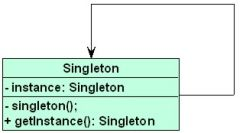
\includegraphics[width=0.5\textwidth]{singletonUML.jpg}
        \centering
    	\label{img:SingletonUML}
     \end{figure}
    
}

%####################################################################
\subsection{\color{colorESCOM}{Ventajas del patr{\' o}n Singleton}}

\begin{itemize}
	{\large
	    \item Un patr{\' o}n Singleton puede escribirse de forma r{\' a}pida y sencilla al no estar poblado de innumerables variables (globales).
	    \item El patr{\' o}n encapsula su creaci{\' o}n, lo que significa que se puede ejercer un control preciso sobre cu{\' a}ndo y c{\' o}mo se accede a {\' e}l.
	    \item Un patr{\' o}n Singleton existente puede derivarse mediante subclases para cumplir nuevas funcionalidades.
	    \item Un Singleton se crea exactamente cu{\' a}ndo se necesita (lazy loading).}
\end{itemize}

%####################################################################

\subsection{\color{colorESCOM}{Desventajas del patr{\' o}n Singleton}}

\begin{itemize}
	{\large
	    \item El uso desinhibido de patr{\' o}n Singleton puede conducir a un estado similar al de la programaci{\' o}n procedimental (no orientada a objetos), y a ensuciar el c{\' o}digo fuente.
	    \item La disponibilidad global de patrones Singleton plantea riesgos si se manejan datos sensibles. Esto pasa debido a que, si se hacen cambios en el Singleton, no se podr{\' a} rastrear qu{\' e} partes del programa est{\' a}n afectadas, lo que dificulta el mantenimiento de software, al ser que los fallos de funcionamiento son dif{\' i}ciles de rastrear. 
	    \item En aplicaciones con muchos usuarios (aplicaciones multiusuario), un patr{\' o}n Singleton puede reducir el rendimiento del programa.}
\end{itemize}

%######################################################

\subsection{\color{colorESCOM}{Implementaci{\' o}n del patr{\' o}n Singleton en Hibernate}}
{\large Para implementar el patr{\' o}n Singleton en Hibernate se debe de crear una clase aparte la cual se encargar{\' a} de la implementaci{\' o}n de un objeto Session Factory de Hibernate como Singleton. 


\vspace{0.5cm}
Debido a que el ``utility class'' es responsable {\' u}nicamente de crear el objeto Session Factory de Hibernate como patr{\' o}n Singleton y retornar dicho objeto, no es necesario la creaci{\' o}n de un objeto adicional para el ``utility class''. 


\vspace{0.5cm}
El constructor del  ``utility class'' debe ser privado, para de esta manera asegurar que ninguna otra clase pueda crear objetos de la sesi{\' o}n de Hibernate.


\vspace{0.5cm}
A continuaci{\' o}n, se presenta un ejemplo de implementaci{\' o}n del patr{\' o}n Singleton en Hibernate:}

\subsubsection{\color{colorESCOM}{HibernateUtility.java}}

    \begin{lstlisting}
        package com.onlinetutorialspoint.config;

        import org.hibernate.SessionFactory;
        import org.hibernate.cfg.Configuration;
        
        public class HibernateUtility {
        
            public static SessionFactory factory;
            //Para no permitir la creacion de objetos a otras clases
        
            private HibernateUtility() {
            }
            //Creando el objeto Hibernate SessionFactory como Singleton
        
            public static synchronized SessionFactory getSessionFactory() {
        
                if (factory == null) {
                    factory = new Configuration().configure("hibernate.cfg.xml").
                            buildSessionFactory();
                }
                return factory;
            }
        }
    \end{lstlisting} 

\pagebreak

\subsubsection{\color{colorESCOM}{Main.java}}

    \begin{lstlisting}
    package com.onlinetutorialspoint.service;
    
    import com.onlinetutorialspoint.config.HibernateUtility;
    import org.hibernate.SessionFactory;
    
    public class Main {
      public static void main(String[] args) {
        SessionFactory sessionFactory = HibernateUtility.getSessionFactory();
        System.out.println("Session Factory : " + sessionFactory.hashCode());
        SessionFactory sessionFactory2 = HibernateUtility.getSessionFactory();
        System.out.println("Session Factory 2 : " + sessionFactory2.hashCode());
        SessionFactory sessionFactory3 = HibernateUtility.getSessionFactory();
        System.out.println("Session Factory 3 : " + sessionFactory3.hashCode());
      }
    }
    \end{lstlisting} 

\pagebreak

%################################################
\section{\color{colorIPN}{Conclusi{\' o}n}}
{\large El patr{\' o}n Singleton es una herramienta bastante poderosa en la programaci{\' o}n orientada objetos, al permitir el ahorro de memoria y recursos durante la ejecuci{\' o}n de una aplicaci{\' o}n cuya programaci{\' o}n este orientada a objetos, al ser que solo permite la creaci{\' o}n de un solo objeto por clase. Adicionalmente la implementaci{\' o}n de aplicaciones con este patr{\' o}n de dise{\~ n}o resulta ser mucho m{\' a}s sencilla y r{\' a}pida.}

\color{colorIPN}{
	\begin{flushright}
		\textit{
			Mauro Sampayo Hern{\' a}ndez
		}
	\end{flushright} \hfill \break
}

\pagebreak

%################################################

\section{\color{colorIPN}{Referencias Bibliogr{\' a}ficas}}
\color{colorESCOM}{
	\begin{thebibliography}{10}
		\bibitem {reference1}
		\newblock {\em Patrones de Dise{\~ n}o Software}
		\newblock \textbf {Inform{\' a}tica PC}
		\newblock [accesed 2021 Jan 02]
		\newblock {\em https://informaticapc.com/patrones-de-diseno/singleton.php}
	
		\bibitem {reference2}
		\newblock {\em Patron singleton: una clase propia}
		\newblock \textbf {Digital Guides IONOS, 2021}
		\newblock [accesed 2021 Jan 02]
		\newblock {\em https://www.baeldung.com/java-request-getsession}
	
		\bibitem {reference3}
		\newblock {\em Singleton Hibernate SessionFactory Example}
		\newblock \textbf {Onlinetutorialspoint, 2015}
		\newblock [accesed 2021 Jan 02]
		\newblock {\em https://www.onlinetutorialspoint.com/hibernate/singleton-hibernate-sessionfactory-example.html}
	\end{thebibliography}
}

\end{document} %##Indica donde termina el documento